\documentclass{standalone}
% pdflatex ts_data.tex
% magick -density 300 ts_data.pdf -quality 90 -resize 640x640 ts_data.png
\usepackage{tikz}
\usetikzlibrary{arrows.meta}

\begin{document}

% Models for time series 
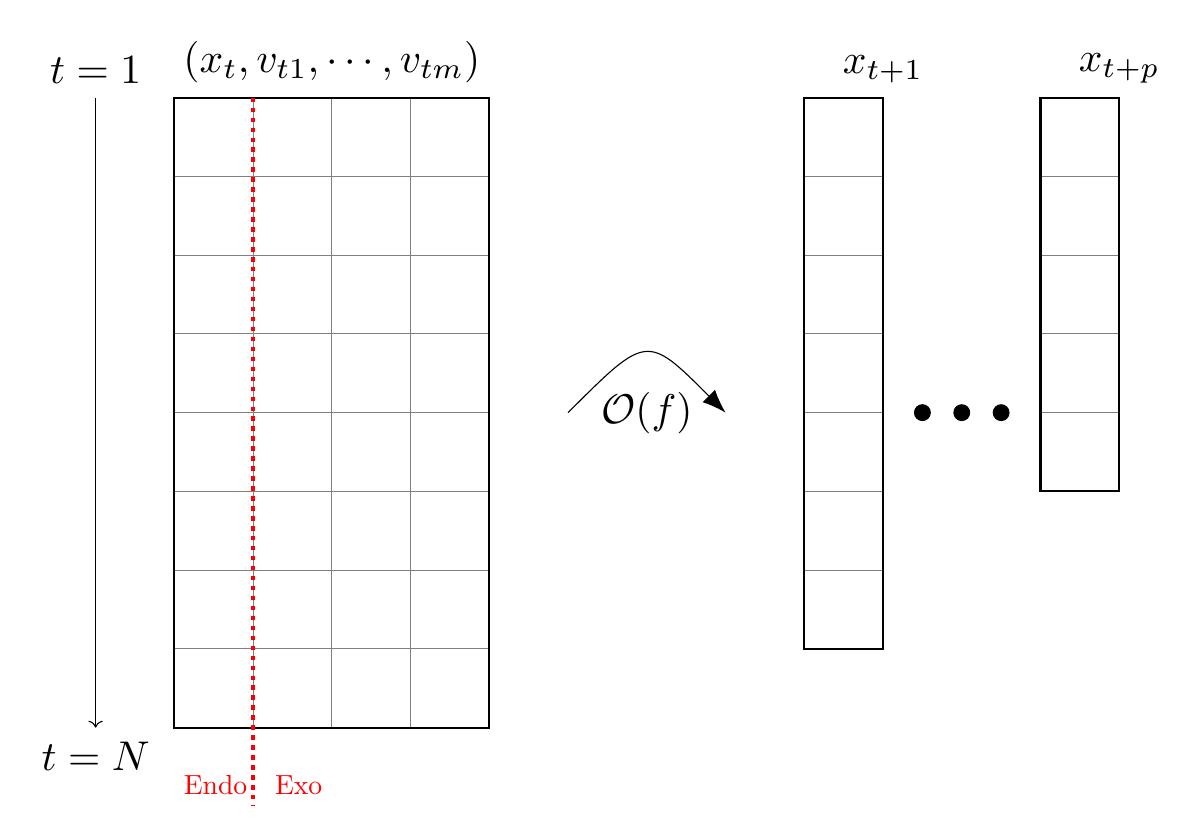
\begin{tikzpicture}

\draw[step=1cm,gray, thin] (0,0) grid (4,8);

\draw[thick, black] (0,0) rectangle (4,8);

\draw[black, ->]
   (-1,8) node[align=left, above, scale=1.5] {$t=1$}
-- (-1, 0) node[align=left, below, scale=1.5] {$t=N$};

\draw[red, dotted, ultra thick] (1,8) -- (1, -1) node[align=center, red, above] {Endo  \,\, Exo};

\draw[-{Latex[length=3mm]}] (5,4) .. controls (6,5) ..  (7, 4);



\draw[step=1cm,gray, thin] (8,1) grid (9,8);
\draw[thick, black] (8,1) rectangle (9,8);



\node[scale=1.5]  at (6,4) (a1) {$\mathcal{O}(f)$};
\node[align=center, above, scale=1.5] at (2,8) (a2)  {$(x_{t}, v_{t1}, \cdots, v_{tm})$};
\node[align=left, above, scale=1.5]  at (9,8) (a3)  {$x_{t+1}$};

\foreach \x in {9.5,10,10.5} 
  \draw[fill] (\x,4) circle (0.1);

\draw[step=1cm,gray, thin] (11,3) grid (12,8);
\draw[thick, black] (11,3) rectangle (12,8);
\node[align=left, above, scale=1.5]  at (12,8) (a4)  {$x_{t+p}$};


\end{tikzpicture}


\end{document}
